%!TEX TS-program = xelatex
\documentclass[]{friggeri-cv}
\usepackage{afterpage}
\usepackage{hyperref}
\usepackage{color}
\usepackage{xcolor}
\hypersetup{
    pdftitle={},
    pdfauthor={},
    pdfsubject={},
    pdfkeywords={},
    colorlinks=false,       % no lik border color
   allbordercolors=white    % white border color for all
}
\addbibresource{bibliography.bib}
\RequirePackage{xcolor}
\definecolor{pblue}{HTML}{0395DE}

\begin{document}
\header{Talip}{Özakça}
      {Computer Engineer}
      
% Fake text to add separator      
\fcolorbox{white}{gray}{\parbox{\dimexpr\textwidth-2\fboxsep-2\fboxrule}{%
.....
}}

% In the aside, each new line forces a line break
\begin{aside}
  \section{Address}
    Yenisehir mah. millet cad. 3981 ada D blok D:15 Pendik / Istanbul
    ~
  \section{Tel \& Skype}
    +90 530 708 1698
    t\_ozakca
    ~
  \section{Mail}
    \href{mailto:mail@talipozakca.com}{\textbf{mail@}\\talipozakca.com}
    \href{mailto:talipozakca@gmail.com}{\textbf{talipozakca@}\\gmail.com}
    ~
  \section{Web \& Git}
    \href{http://www.talipozakca.com}{talipozakca.com}
    \href{https://github.com/talipozakca}{github.com/talipozakca}
    ~
  \section{Languages}
    \textbf{Turkish}&
\includegraphics[scale=0.40]{img/5stars.png}
    \textbf{English}&
\includegraphics[scale=0.40]{img/4stars.png}
    \textbf{German}&
\includegraphics[scale=0.40]{img/2stars.png}
    ~
  \section{Programming}
    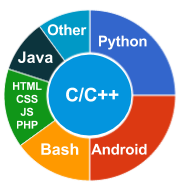
\includegraphics[scale=0.62]{img/programming.png}
    ~
    \section{Computer Skills}
    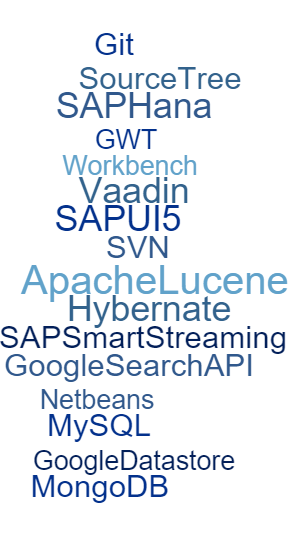
\includegraphics[scale=0.62]{img/skills.png}
    ~
  \section{OS Preference}
    \textbf{MacOS}&
\includegraphics[scale=0.40]{img/5stars.png}
    \textbf{Windows}&
\includegraphics[scale=0.40]{img/4stars.png}
    \textbf{GNU/Linux}&
\includegraphics[scale=0.40]{img/4stars.png}
    ~
\end{aside}

\section{Experience}
\begin{entrylist}
  \entry
    {10/13 - Now}
    {Software Developer}
    {SAP, Istanbul, Turkey}
    {
     \textbf{SAP Hana Vora - Disk Engine:} Disk engine side of the distributed in memory database system SAP Hana Vora. I am currently a scrum master in our core development team which uses agile methodology for development.
    \item \textbf{SAP Education Platform:} SAP Education Platform is a project which aims to digitialize the education processes and ease the communication among the students, parents and the teachers.
    \item \textbf{SAP IT Operations Analytics (ITOA):} Developing the new analytics solution of SAP for realtime log analysis for IT operations.\\
    \item \textbf{Keywords: Data Streaming, Java, Front-end Developer, JavaScript, Scrum Master\\}
    }
  \entry
    {07/12 – 08/12 }
    {Intern}
    {AKGÜN YAZILIM, Ankara, Turkey}
    {In the project “HBYS” (Hospital Information Management System) I prepared a report about upgrading the ExtJs Framework version.\\\\
    \textbf{Keywords: JavaScript, ExtJs\\}}
    \entry
    {12/09 - 06/09}
    {Intern}
    {VARDAR YAZILIM DANIŞMANLIK, Ankara, Turkey}
    {Research and basic implementation with using Vaadin to get familiar with company products. Implemetation of runtime dynamic reports part of the project ActivWorks with using JasperReports.\\\\
    \textbf{Keywords: Java, Vaadin, Dynamic Reports\\}
    }
\end{entrylist}

\section{Education}
\begin{entrylist}
  \entry
    {09/08 - 06/13}
    {B. Sc. in Computer Engineering}
    {Ihsan Doğramacı Bilkent University, Turkey}
    {Engineering Faculty, Computer Engineering (English)\\
    2.91/4.00 \\}
    \entry
    {01/12 - 06/12}
    {B. Sc. in Computer Engineering}
    {Kungliga Tekniska Högskolan, Sweden }
    {Computational Science and Communications, Computer Science (English)\\
    Erasmus Exchange Student \\}

\end{entrylist}

\section{Certifications}
\begin{entrylist}
  \entry
    {06/15}
    {Communication Skills}
    {PDS (Performance Development Services)}
    {\emph{}}
    \entry
    {04/14}
    {Design Thinking Workshop}
    {Hasso-Plattner-Institute}
    {\emph{}}
\end{entrylist}

\newpage

\begin{aside}
~
~
~
  \section{Places Lived}
    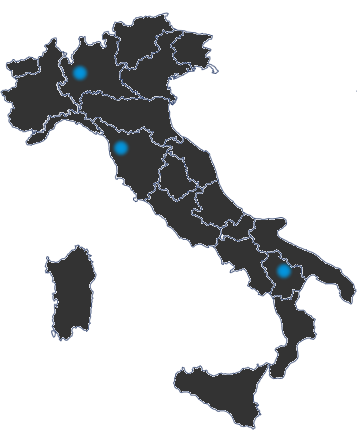
\includegraphics[scale=0.25]{img/italia.png}
    ~
  \section{Languages}
    \textbf{Italian}
\includegraphics[scale=0.40]{img/5stars.png}
    \textbf{English}
\includegraphics[scale=0.40]{img/4stars.png}
    ~
  \section{Personal Skills}
    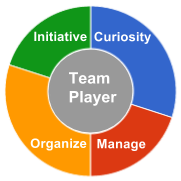
\includegraphics[scale=0.62]{img/personal.png}
    ~
\end{aside}

\section{Publications}
C. Benedetto, E. Mingozzi, C. Vallati\\
\textbf{A Handoff Algorithm based on Link Quality Prediction for Mass Transit Wireless Mesh Networks}\\
\emph{Proceedings of the 18th IEEE Symposium on Computers and Communications (ISCC 2013), Split, Croatia, July 7-10, 2013}
\\
\section{Other Info}
For the Italian job market:\\
\emph{Si autorizza il trattamento delle informazioni contenute nel curriculum in conformità alle disposizioni previste dal d.lgs. 196/2003. Si dichiara altresì di essere consapevole che, in caso di dichiarazioni non veritiere, si è passibili di sanzioni penali ai sensi del DPR 445/00 oltre alla revoca dei benefici eventualmente percepiti.}
\\
\begin{flushleft}
\emph{January 14th, 2014}
\end{flushleft}
\begin{flushright}
\emph{Carmine Benedetto}
\end{flushright}

%%% This piece of code has been commented by Karol Kozioł due to biblatex errors. 
% 
%\printbibsection{article}{article in peer-reviewed journal}
%\begin{refsection}
%  \nocite{*}
%  \printbibliography[sorting=chronological, type=inproceedings, title={international peer-reviewed conferences/proceedings}, notkeyword={france}, heading=subbibliography]
%\end{refsection}
%\begin{refsection}
%  \nocite{*}
%  \printbibliography[sorting=chronological, type=inproceedings, title={local peer-reviewed conferences/proceedings}, keyword={france}, heading=subbibliography]
%\end{refsection}
%\printbibsection{misc}{other publications}
%\printbibsection{report}{research reports}

\end{document}
